
\section{The Prototype}
\label{sec:overview}

This section presents the developed prototype, discussing its architecture (Section~\ref{sec:architecture}), implementation issues (Section~\ref{sec:implementation}), deployment procedures (Section~\ref{sec:instalation}), and usage examples (Section~\ref{sec:using}).

\subsection{Architectural Overview}
\label{sec:architecture}

Fig.~\ref{fig:prototype-overview-simple} provides a conceptual overview of the prototype and its main components.
The text recognition applications provide the components responsible for recognizing the text found within detected regions. The text spotting module includes container applications that encapsulate the text spotting methods related to deliverables E2 and E3. The post-processing module comprises two containers: the post-processing method developed by the Samsung Research (SRBR) team, and an improved version developed at Unicamp. Similarly, the text recognition module provides three containers that encapsulate the three recognition methods presented in deliverable E3: Tesseract, Long Short-Term Memory (LSTM), and Convolutional Recurrence Neural Network (CRNN) recognition methods.

Table~\ref{tab:methods-available} summarizes the text detection and recognition methods handled in the prototype. As we can observe, we consider non-deep and deep-learning-based solutions.\footnote{Readers may refer to Deliverables E1 and E3 to find descriptions of such methods.}
%
\begin{table}[H]
    \centering
    \caption{Method for text detection and recognition available in the prototype.}
    \label{tab:methods-available}
    \begin{tabular}{ll|p{5.5cm}}
        \hline
        \topline
        \headcol
        \textbf{Type}   & \textbf{Methods for Text Detection}       & \textbf{Methods for Text Recognition} \\ \midline
        & - SnooperText                             	& - Tesseract v.3                         \\
        & - Canny Text Detection                    & - Tesseract with Post-processing provided \\
        & - MSER-SWT Text Detection                 &   by Samsung Team   \\
        & - Multi-Lingual Text Detection            & - Tesseract with Improved Post-processing \\
        & - FASText                                 &                                       \\
        
        \ml{-6}{*}{Non-Deep Methods}
        & - Scene Text Recognition (pretrained models) &                                       \\ \hline \hline
        & - SSTD                                       & - LSTM (Tesseract v.4)                  \\
        & - TextBoxes                                  & - CRNN                                  \\
        & - TextBoxes++                                &                                       \\
        & - SSD-MobilenetV2                            &                                       \\
        & - YOLOv3                                     &                                       \\
        
        \ml{-6}{*}{Deep Learning-Based 
            Methods}        & - SqueezeDet                                 &                                       \\
        \bottomlinec
    \end{tabular}
\end{table}
\footnotesize{$^{\star}$Some components are not fully integrated to the prototype as a docker application. We will provide a Dockerfile for all these components soon.}


\subsection{Implementation Overview}
\label{sec:implementation}


The prototype developed in this deliverable contains several applications with different software dependencies, including libraries, programming tools, and the base operating system. The integration of all these pieces of software into a single prototype is very challenging and we opted to package all applications that compose the prototype using the Docker\footnote{\url{https://www.docker.com/} (As of Dec. 2018).} technology. Docker is an open source platform (Apache License 2.0) for operating-system-level virtualization. Docker provides a standardized unit software for packaging the source code and all its dependencies, including system tools, system libraries, and settings.

In this prototype, we implement \textit{Dockerfiles} that automatically package the source code, install its dependencies, install and compile source codes, and finally builds a docker image able to run the application as a command line, in a proper software platform. Fig.~\ref{fig:overview-prototype} illustrates an overview of the architecture of the prototype. We built two base docker images, which contain some common libraries required for running non-deep- and deep-learning-based methods. These base docker images are used to build the docker images for the applications.
%
\begin{figure}
    \centering
    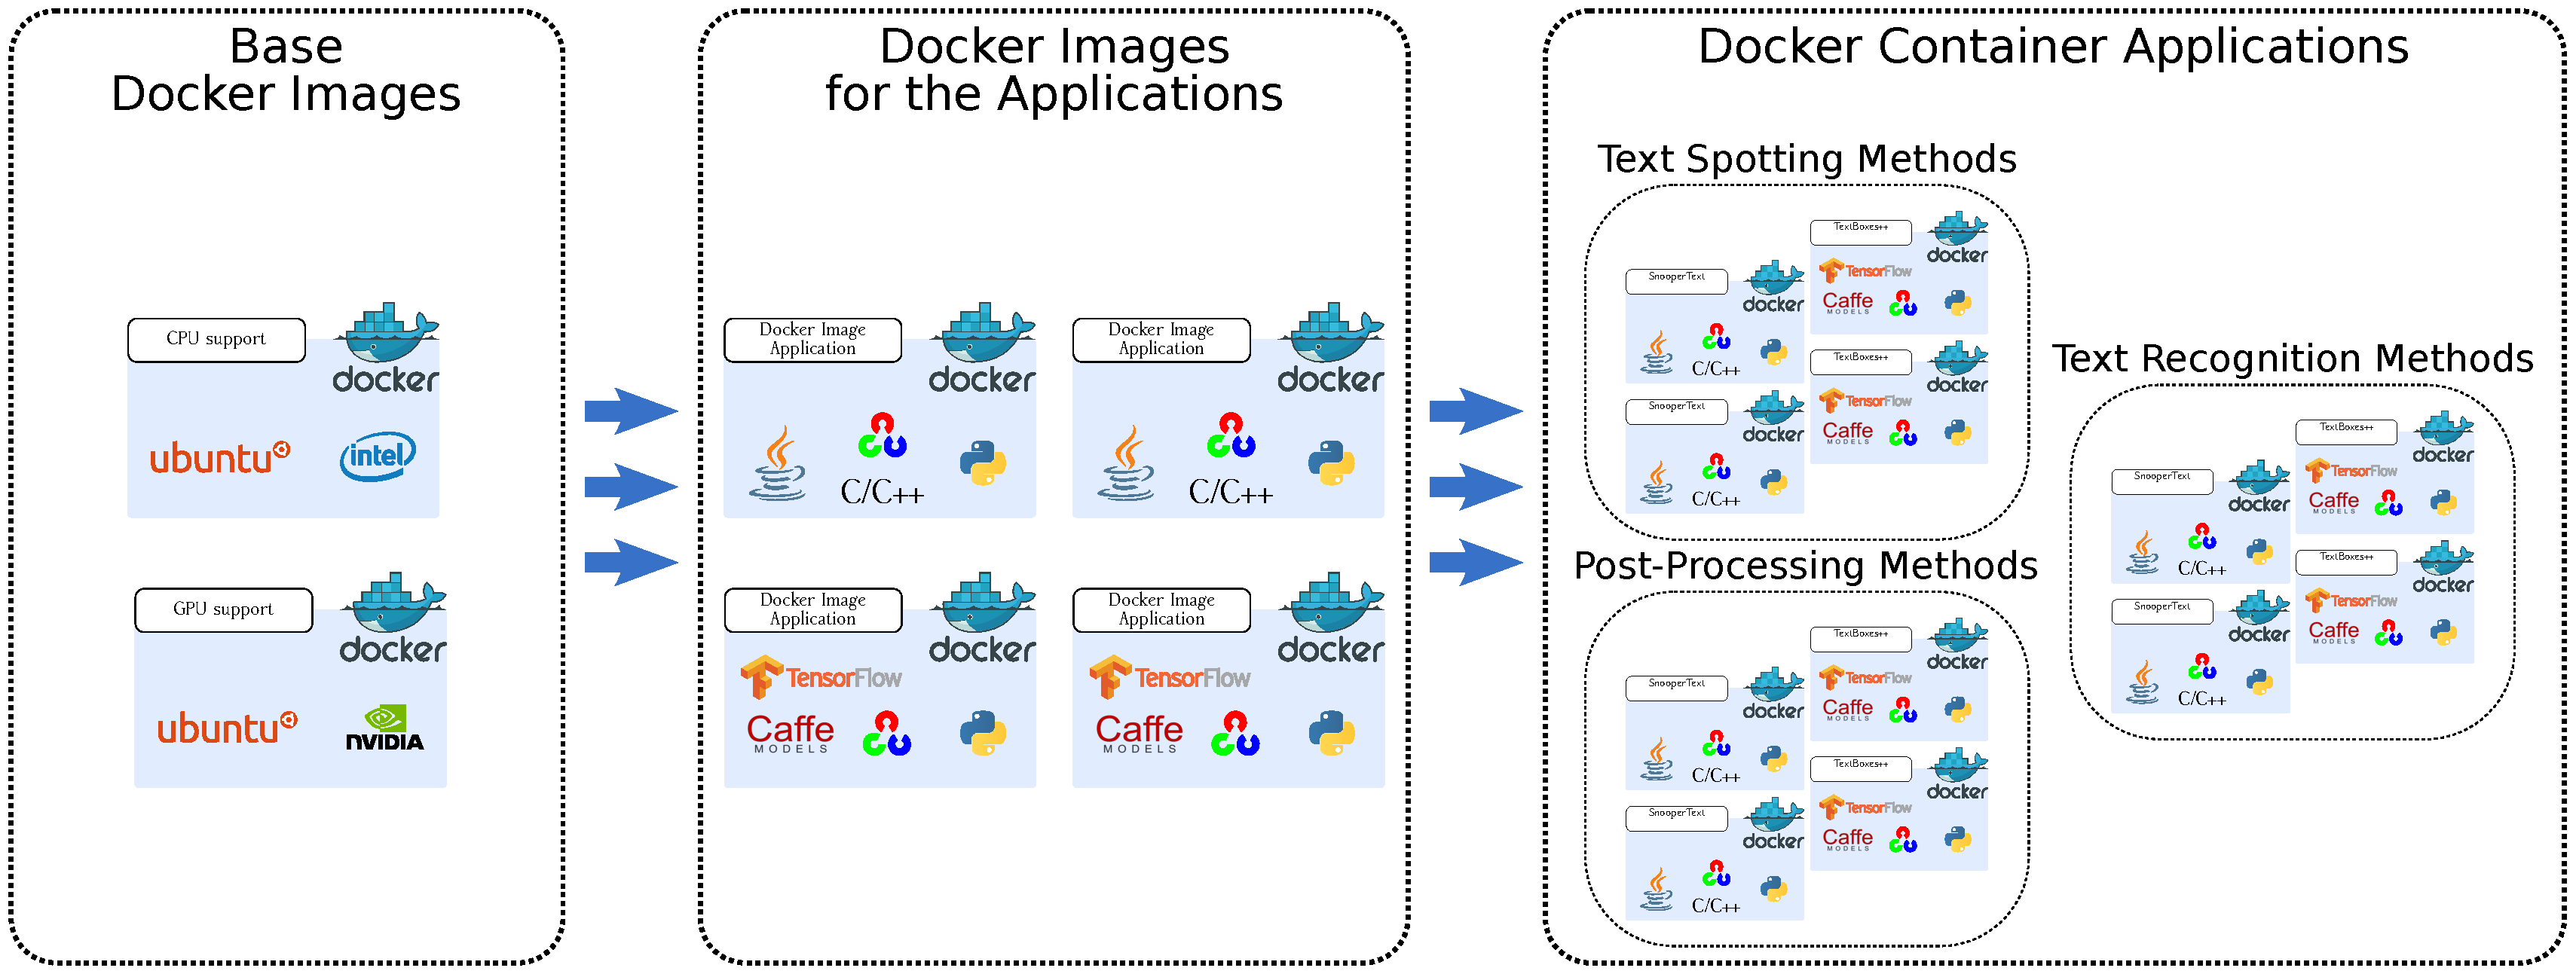
\includegraphics[width=0.98\textwidth]{figs/prototype-overview.pdf}
    \caption{Architectural overview of the prototype.}
    \label{fig:overview-prototype}
\end{figure}


\subsection{Deploying the Prototype}
\label{sec:instalation}

This section presents the procedures for deploying the prototype.

\subsubsection{How to Build the Docker Base Images}
\label{sec:build-docker-base-images}

We provide Dockerfiles for all docker containers used in this prototype. Specially, we built two Dockerfiles, which are used as base for all components of the prototype. With this, we reduce the time to generate the docker containers and we standardize some common software, tools and libraries (e.g., OpenCV, CUDA, OpenBLAS).

Suppose that the environment variable \textsc{ROOT\_DIR} points to the path where the prototype was downloaded. To build the docker base images, the following commands can be used:
%
\begin{lstlisting}[style=fancyterminal]
 $ cd $ROOT_DIR
 $ ./0-main-build-docker-base-images.sh
\end{lstlisting}

This shell script calls the scripts responsible for building the docker base images, whose Dockerfiles are located in \textsc{\$ROOT\_DIR/misc/base-dockerfiles} directory. To see if the base images were built correctly, the command \emph{\$ docker images} may be used. As result of its use, two docker images, named as \textit{unicamp-mltsr-deliverable-e4/base-cpu-support:4.0} and \textit{unicamp-mltsr-deliverable-e4/base-gpu-support:4.0}, are identified (see listing below).

\begin{lstlisting}[style=fancyterminal]
 REPOSITORY                                        TAG                     IMAGE ID    
 unicamp-mltsr-deliverable-e4/base-cpu-support     4.0                     d822492254bf
 unicamp-mltsr-deliverable-e4/base-gpu-support     4.0                     d9cad4ce0273
 ubuntu                                            16.04                   b0ef3016420a
 nvidia/cuda                                       8.0-devel-ubuntu16.04   d610c8c58845
\end{lstlisting}



\subsubsection{How to Build the Docker Image Applications}
\label{sec:build-docker-image-app}

The Docker Image Applications form the most important component in our prototype, since they contain the implementation source code (and its compiled version) of text detection and recognition methods. Those applications contain the \textsc{ENTRYPOINT} of their respective docker container. The \textsc{ENTRYPOINT} is a Dockerfile instruction used to set the image's main command in such a way that a docker container can be run by means of a command line in a Linux terminal. The Dockerfiles also contain the instruction needed to install the software requirements of the applications and also instructions to automatically compile the source code. Therefore, there is no need for the direct use of docker containers to compile libraries and source codes manually.

To build the docker images needed to run the applications, the following command in the terminal can be used:
%
\begin{lstlisting}[style=fancyterminal]
 $ ./0-main-build-docker-images-text-spotting.sh
 $ ./0-main-build-docker-images-text-recognition.sh
 $ ./0-main-build-docker-images-post-processing.sh
 $ ./0-main-build-docker-images-evaluations.sh
\end{lstlisting}

These shell scripts call the scripts responsible for building the docker images that contain the text spotting, post-processing, text recognition methods, as well as the docker containers used to evaluate the text spotting and text recognition methods. To see if the docker images were built correctly, the command \emph{\$ docker images} may be used to have access to information regarding the built docker images. We provided a demo script (\textit{demo-00-testing-build-docker-images.sh}) that builds all docker images required to use this prototype.

\subsection{Using the Prototype}
\label{sec:using}

\subsubsection{Running a Text Spotting Application}

We provide shell scripts to run a text spotting application by choosing the method to be used to detect the candidate regions and also to run all text spotting methods available in this prototype. The option to run post-processing methods on top of text spotting method's output is also available.  

To run all text spotting methods available, the following command can be used:

\begin{lstlisting}[style=fancyterminal]
 $ ./1-main-text-spotting-methods.sh \
        --dataset_path /path/to/datasets \
        --working_path /path/to/working/directory/ \
        --dataset_id icdarXX \
        --text_spotting_method_id all-methods
\end{lstlisting}

To see all options available, the following command can be used:
\begin{lstlisting}[style=fancyterminal]
 $ ./1-main-text-spotting-methods.sh --help
 Usage: ./1-main-text-spotting-methods.sh [options]
 
 options:
 -h, --help                show brief help
 --dataset_path            path to dataset directory
 --working_path            path to output directory
 --dataset_id              dataset identifier (choose from icdar11, icdar13, icdar15)
 --text_spotting_method_id text spotting method identifier (choose from options below)
       options:
           all-methods (default)
           deliverable-e2-canny
           deliverable-e2-snoopertext
           deliverable-e4-canny
           deliverable-e4-snoopertext
           deliverable-e4-mserswt
           deliverable-e4-multiligual
           deliverable-e4-scenetext
           deliverable-e4-ssd-mobilenetv2
           deliverable-e4-sstd
           deliverable-e4-squeezedet
           deliverable-e4-yolov3
\end{lstlisting}

To run the post-processing methods available on top of all text spotting methods, the following command can be used:

\begin{lstlisting}[style=fancyterminal]
 $ ./2-main-postprocessing.sh  
        --dataset_path /path/to/datasets \
        --working_path /path/to/working/directory/ \
        --dataset_id icdarXX \
        --text_spotting_method_id all-methods \
        --postprocessing_method_id all-methods
\end{lstlisting}

To see all options available, the following command can be used:
\begin{lstlisting}[style=fancyterminal]
 $ ./2-main-postprocessing.sh --help
 Usage: ./2-main-postprocessing.sh [options]
 
 options:
 -h, --help                show brief help
 --dataset_path            path to dataset directory
 --working_path            path to output directory
 --dataset_id              dataset identifier (choose from icdar11, icdar13, icdar15)
 --text_spotting_method_id text spotting method identifier (choose from options below)
       options:
           all-methods (default)
           deliverable-e2-canny
           deliverable-e2-snoopertext
           deliverable-e4-canny
           deliverable-e4-snoopertext
           deliverable-e4-mserswt
           deliverable-e4-multiligual
           deliverable-e4-scenetext
           deliverable-e4-ssd-mobilenetv2
           deliverable-e4-sstd
           deliverable-e4-squeezedet
           deliverable-e4-yolov3
 --postprocessing_method_id post-processing method identifier (choose from options below)
       options:
           all-methods (default)
           postprocessing-samsung
           postprocessing-improved
\end{lstlisting}

Finally, to evaluate the localizations obtained with text spotting methods, as well as the improvements obtained with the post-processing methods, the following command can be used:
\begin{lstlisting}[style=fancyterminal]
 $ ./4-main-spotting-evaluation.sh 
        --dataset_path /path/to/datasets \
        --working_path /path/to/working/directory/ \
        --dataset_id icdarXX \
        --text_spotting_method_id all-methods \
        --postprocessing_method_id all-methods
\end{lstlisting}

To see all options available, the following command can be used:
\begin{lstlisting}[style=fancyterminal]
 $ ./4-main-spotting-evaluation.sh --help
 Usage: ./4-main-spotting-evaluation.sh [options]
 
 options:
 -h, --help                show brief help
 --dataset_path            path to dataset directory
 --working_path            path to output directory
 --dataset_id              dataset identifier (choose from icdar11, icdar13, icdar15)
 --text_spotting_method_id text spotting method identifier (choose from options below)
       options:
           all-methods (default)
           deliverable-e2-canny
           deliverable-e2-snoopertext
           deliverable-e4-canny
           deliverable-e4-snoopertext
           deliverable-e4-mserswt
           deliverable-e4-multiligual
           deliverable-e4-scenetext
           deliverable-e4-ssd-mobilenetv2
           deliverable-e4-sstd
           deliverable-e4-squeezedet
           deliverable-e4-yolov3
 --postprocessing_method_id post-processing method identifier (choose from options below)
       options:
           all-methods (default)
           none
           postprocessing-improved
           postprocessing-samsung
\end{lstlisting}



\subsubsection{Running an End-to-End Recognition Application}

We also provide a shell script to run an end-to-end solution by choosing the text spotting methods used to detect the candidate regions, the post-processing method to improve the text detection rates, and the text recognition methods used to determine the texts found within detected candidate regions.

Assume that the execution of a text spotting application was performed as described in the previous section. To run the text recognition methods, available in this prototype, on top of the text spotting results, the following command can be used:

\begin{lstlisting}[style=fancyterminal]
 $ ./3-main-recognition.sh \
        --dataset_path /path/to/datasets \
        --working_path /path/to/working/directory/ \
        --dataset_id icdarXX \
        --text_spotting_method_id all-methods \
        --postprocessing_method_id all-methods \
        --text_recognition_method_id all-methods
\end{lstlisting}

To see all options available, the following command can be used:

\begin{lstlisting}[style=fancyterminal]
 $ ./3-main-recognition.sh --help
 Usage: ./3-main-recognition.sh [options]
 
 options:
 -h, --help                show brief help
 --dataset_path            path to dataset directory
 --working_path            path to output directory
 --dataset_id              dataset identifier (choose from icdar11, icdar13, icdar15)
 --text_spotting_method_id text spotting method identifier (choose from options below)
       options:
           all-methods (default)
           deliverable-e2-canny
           deliverable-e2-snoopertext
           deliverable-e4-canny
           deliverable-e4-snoopertext
           deliverable-e4-mserswt
           deliverable-e4-multiligual
           deliverable-e4-scenetext
           deliverable-e4-ssd-mobilenetv2
           deliverable-e4-sstd
           deliverable-e4-squeezedet
           deliverable-e4-yolov3
 --postprocessing_method_id post-processing method identifier (choose from options below)
       options:
           all-methods (default)
           none
           postprocessing-improved
           postprocessing-samsung
 --text_recognition_method_id recognition method identifier (choose from options below)
       options:
           all-methods (default)
           deliverable-e4-tesseract
           deliverable-e4-lstm
           deliverable-e4-crnn
\end{lstlisting}


Finally, to evaluate the recognition methods executed on top of all text recognition methods, as well as the improvements obtained with the post-processing methods, the following command can be used:
\begin{lstlisting}[style=fancyterminal]
 $ ./4-main-recognition-evaluation.sh 
        --dataset_path /path/to/datasets \
        --working_path /path/to/working/directory/ \
        --dataset_id icdarXX \
        --text_spotting_method_id all-methods \
        --postprocessing_method_id all-methods \
        --text_recognition_method_id all-methods
\end{lstlisting}

To see all options available, the following command can be used:
\begin{lstlisting}[style=fancyterminal]
 $ ./4-main-recognition-evaluation.sh --help
 Usage: ./4-main-recognition-evaluation.sh [options]
 
 options:
 -h, --help                show brief help
 --dataset_path            path to dataset directory
 --working_path            path to output directory
 --dataset_id              dataset identifier (choose from icdar11, icdar13, icdar15)
 --text_spotting_method_id text spotting method identifier (choose from options below)
       options:
           all-methods (default)
           deliverable-e2-canny
           deliverable-e2-snoopertext
           deliverable-e4-canny
           deliverable-e4-snoopertext
           deliverable-e4-mserswt
           deliverable-e4-multiligual
           deliverable-e4-scenetext
           deliverable-e4-ssd-mobilenetv2
           deliverable-e4-sstd
           deliverable-e4-squeezedet
           deliverable-e4-yolov3
 --postprocessing_method_id post-processing method identifier (choose from options below)
       options:
           all-methods (default)
           none
           postprocessing-improved
           postprocessing-samsung
 --text_recognition_method_id recognition method identifier (choose from options below)
       options:
           all-methods (default)
           deliverable-e4-tesseract
           deliverable-e4-lstm
           deliverable-e4-crnn

\end{lstlisting}


\section{Usage Scenarios}
\label{sec:usage-scenario}

In this section, we provide an overview of a possible usage of the prototype considering scenarios, in which a user wants to reproduce the results of a text spotting and text recognition solution, both with and without the use of post-processing methods. We also provide these and other demos along with prototype. Hereinafter, we are assuming that all images were built as described in Sections~\ref{sec:build-docker-base-images}~and~\ref{sec:build-docker-image-app}, and that dataset to be used is located in {\footnotesize \ttfamily /dataset/ICDAR11/TEXT\_LOCALIZATION/TEST/Challenge1\_Test\_Task12\_Images}.

\subsection{Running the Snooper Text Detection combined with Tesseract recognition method.}

To run the Snooper Text Detection, the following command can be used:
\begin{lstlisting}[style=fancyterminal]
 $ ./1-main-text-spotting-methods.sh \
    --dataset_path /dataset/ICDAR11/TEXT_LOCALIZATION/TEST/Challenge1_Test_Task12_Images \
    --working_path /working \
    --dataset_id icdar11 \
    --text_spotting_method_id deliverable-e2-snoopertext

\end{lstlisting}

To run the Improved post-processing provided by the Unicamp Team, the following command can be used:

\begin{lstlisting}[style=fancyterminal]
 $ ./2-main-postprocessing.sh \
    --dataset_path /dataset/ICDAR11/TEXT_LOCALIZATION/TEST/Challenge1_Test_Task12_Images \
    --working_path /working \
    --dataset_id icdar11 \
    --text_spotting_method_id deliverable-e2-snoopertext \
    --postprocessing_method_id postprocessing-improved
\end{lstlisting}

To run the Tesseract recognizer on top of the raw localizations detected by the Snooper Text Detection, the following command can be used:
\begin{lstlisting}[style=fancyterminal]
 $ ./3-main-recognition.sh \
    --dataset_path /dataset/ICDAR11/TEXT_LOCALIZATION/TEST/Challenge1_Test_Task12_Images \
    --working_path /working \
    --dataset_id icdar11 \
    --text_spotting_method_id deliverable-e2-snoopertext \
    --postprocessing_method_id none \
    --text_recognition_method_id deliverable-e4-tesseract
\end{lstlisting}

To evaluate the performance results for the text spotting task without post-processing, the following command can be used:
\begin{lstlisting}[style=fancyterminal]
 $ ./4-main-spotting-evaluation.sh \
    --dataset_path /dataset/ICDAR11/TEXT_LOCALIZATION/TEST/Challenge1_Test_Task12_Images \
    --working_path /working \
    --dataset_id icdar11 \
    --text_spotting_method_id deliverable-e4-snoopertext \
    --postprocessing_method_id none
\end{lstlisting}

To evaluate the performance results for the text spotting task with post-processing, the following command can be used:
\begin{lstlisting}[style=fancyterminal]
 $ ./4-main-spotting-evaluation.sh \
    --dataset_path /dataset/ICDAR11/TEXT_LOCALIZATION/TEST/Challenge1_Test_Task12_Images \
    --working_path /working \
    --dataset_id icdar11 \
    --text_spotting_method_id deliverable-e2-snoopertext \
    --postprocessing_method_id postprocessing-improved
\end{lstlisting}

Finally, to evaluate the performance results for the text recognition task with post-processing, the following command can be used:
\begin{lstlisting}[style=fancyterminal]
 $ ./4-main-recognition-evaluation.sh \
    --dataset_path /dataset/ICDAR11/TEXT_LOCALIZATION/TEST/Challenge1_Test_Task12_Images \
    --working_path /working \
    --dataset_id icdar11 \
    --text_spotting_method_id deliverable-e2-snoopertext \
    --postprocessing_method_id postprocessing-improved \
    --text_recognition_method_id deliverable-e4-tesseract
\end{lstlisting}

\subsection{Running the Scene Text Recognition combined with Tesseract recognition method.}

To run the Scene Text Detection, please use the following command:
\begin{lstlisting}[style=fancyterminal]
 $ ./1-main-text-spotting-methods.sh \
    --dataset_path /dataset/ICDAR11/TEXT_LOCALIZATION/TEST/Challenge1_Test_Task12_Images \
    --working_path/working \
    --dataset_id icdar11 \
    --text_spotting_method_id deliverable-e4-scenetext
\end{lstlisting}

To run the Post-processing provided by the Samsung Team with Tesseract Recognition methods, the following command can be used:
\begin{lstlisting}[style=fancyterminal]
 $ ./2-main-postprocessing.sh \
    --dataset_path /dataset/ICDAR11/TEXT_LOCALIZATION/TEST/Challenge1_Test_Task12_Images \
    --working_path/working \
    --dataset_id icdar11 \
    --text_spotting_method_id deliverable-e4-scenetext \
    --postprocessing_method_id postprocessing-samsung
\end{lstlisting}

To run the Tesseract recognizer on top of the raw localizations detected by the Scene Text Detection, the following command can be used:
\begin{lstlisting}[style=fancyterminal]
 $ ./3-main-recognition.sh \
    --dataset_path /dataset/ICDAR11/TEXT_LOCALIZATION/TEST/Challenge1_Test_Task12_Images \
    --working_path/working \
    --dataset_id icdar11 \
    --text_spotting_method_id deliverable-e4-scenetext \
    --postprocessing_method_id none \
    --text_recognition_method_id deliverable-e4-tesseract
\end{lstlisting}

To evaluate the performance results for the text spotting task without post-processing, the following command can be used:
\begin{lstlisting}[style=fancyterminal]
 $ ./4-main-spotting-evaluation.sh \
    --dataset_path /dataset/ICDAR11/TEXT_LOCALIZATION/TEST/Challenge1_Test_Task12_Images \
    --working_path/working \
    --dataset_id icdar11 \
    --text_spotting_method_id deliverable-e4-scenetext \
    --postprocessing_method_id none
\end{lstlisting}

To evaluate the performance results for the text spotting task with post-processing, the following command can be used:
\begin{lstlisting}[style=fancyterminal]
 $ ./4-main-spotting-evaluation.sh \
    --dataset_path /dataset/ICDAR11/TEXT_LOCALIZATION/TEST/Challenge1_Test_Task12_Images \
    --working_path/working \
    --dataset_id icdar11 \
    --text_spotting_method_id deliverable-e4-scenetext \
    --postprocessing_method_id postprocessing-samsung
\end{lstlisting}

Finally, to evaluate the performance results for the text recognition task with post-processing, the following command can be used:
\begin{lstlisting}[style=fancyterminal]
 $ ./4-main-recognition-evaluation.sh \
    --dataset_path /dataset/ICDAR11/TEXT_LOCALIZATION/TEST/Challenge1_Test_Task12_Images \
    --working_path /working \
    --dataset_id icdar11 \
    --text_spotting_method_id deliverable-e4-scenetext \
    --postprocessing_method_id postprocessing-samsung \
    --text_recognition_method_id deliverable-e4-tesseract
\end{lstlisting}


\subsection{Running the SSTD Text Detection combined with LSTM recognition method.}

To run the SSTD Text Detection, the following command can be used:
\begin{lstlisting}[style=fancyterminal]
 $ ./1-main-text-spotting-methods.sh \
    --dataset_path /dataset/ICDAR11/TEXT_LOCALIZATION/TEST/Challenge1_Test_Task12_Images \
    --working_path/working \
    --dataset_id icdar11 \
    --text_spotting_method_id deliverable-e4-sstd
\end{lstlisting}

To run the Post-processing provided by the Samsung Team with Tesseract Recognition methods, the following command can be used:
\begin{lstlisting}[style=fancyterminal]
 $ ./2-main-postprocessing.sh \
    --dataset_path /dataset/ICDAR11/TEXT_LOCALIZATION/TEST/Challenge1_Test_Task12_Images \
    --working_path/working \
    --dataset_id icdar11 \
    --text_spotting_method_id deliverable-e4-sstd \
    --postprocessing_method_id postprocessing-samsung
\end{lstlisting}

To run the LSTM recognizer on top of the raw regions detected by the SSTD Text Detection method, the following command can be used:
\begin{lstlisting}[style=fancyterminal]
 $ ./3-main-recognition.sh \
    --dataset_path /dataset/ICDAR11/TEXT_LOCALIZATION/TEST/Challenge1_Test_Task12_Images \ 
    --working_path /working \ 
    --dataset_id icdar11 \ 
    --text_spotting_method_id deliverable-e4-sstd \
    --postprocessing_method_id none
    --text_recognition_method_id deliverable-e4-lstm
\end{lstlisting}

Otherwise, use the \textit{--postprocessing\_method\_id} parameter to enable the recognition from the text detection results improved by the post-processing method:

\begin{lstlisting}[style=fancyterminal]
 $ ./3-main-recognition.sh \
    --dataset_path /dataset/ICDAR11/TEXT_LOCALIZATION/TEST/Challenge1_Test_Task12_Images \ 
    --working_path /working \ 
    --dataset_id icdar11 \ 
    --text_spotting_method_id deliverable-e4-sstd \ 
    --postprocessing_method_id postprocessing-samsung \ 
    --text_recognition_method_id deliverable-e4-lstm
\end{lstlisting}

To evaluate the performance results for the text spotting task without post-processing, the following command can be used:
\begin{lstlisting}[style=fancyterminal]
 $ ./4-main-spotting-evaluation.sh \
    --dataset_path /dataset/ICDAR11/TEXT_LOCALIZATION/TEST/Challenge1_Test_Task12_Images \
    --working_path/working \
    --dataset_id icdar11 \
    --text_spotting_method_id deliverable-e4-sstd \
    --postprocessing_method_id none
\end{lstlisting}

To evaluate the performance results for the text spotting task with post-processing, the following command can be used:
\begin{lstlisting}[style=fancyterminal]
 $ ./4-main-spotting-evaluation.sh \
    --dataset_path /dataset/ICDAR11/TEXT_LOCALIZATION/TEST/Challenge1_Test_Task12_Images \
    --working_path/working \
    --dataset_id icdar11 \
    --text_spotting_method_id deliverable-e4-sstd \
    --postprocessing_method_id postprocessing-samsung
\end{lstlisting}

Finally, to evaluate the performance results for the text recognition task with post-processing, the following command can be used:
\begin{lstlisting}[style=fancyterminal]
 $ ./4-main-recognition-evaluation.sh \
    --dataset_path /dataset/ICDAR11/TEXT_LOCALIZATION/TEST/Challenge1_Test_Task12_Images \
    --working_path /working \
    --dataset_id icdar11 \
    --text_spotting_method_id deliverable-e4-sstd \
    --postprocessing_method_id postprocessing-samsung \
    --text_recognition_method_id deliverable-e4-lstm
\end{lstlisting}


\section{Conclusions}
\label{sec:conclusions}

This report refers to the fourth deliverable related to the project Multi-Lingual Text Spotting and Recognition (MLTSR). The report describes the developed prototype which supports both text detection and end-to-end recognition tasks. Two types of approaches were considered in the implementation of text detection and recognition approaches: methods that do not rely on deep learning strategies; and methods that take advantage of deep-learning-based architectures. The prototype also includes post-processing components, which may be used to improve text detection results. 

The implementation of the prototype considered a docker-based infrastructure, which integrates programming tools, source codes, and even the base operating system. We believe that the adopted prototype organization, therefore, provides an unified infrastructure for the development, implementation, evaluation, and usage of text detection and recognition methods.

The construction of the prototype provided insights about traditional and recently proposed approaches for the text detection and recognition problems, opening promising research directions for the MSTSR project.
Some possible future work may encompass:

\begin{enumerate}

    \item Extend the prototype to encapsulate different evaluation protocols, including, among others, datasets, and performance evaluation metrics. One starting point might be the datasets and benchmarks listed in the survey provided as Deliverable E1.
    
    \item Extend the prototype to simulate scenarios commonly found when handling restrictive computing devices. This infrastructure may contribute, for example, to speed up the development of new text localization and recognition methods customized for specific constrained hardware configurations.
    
    \item Extend the prototype to include a graphical user interface, which would support the selection of text detection and recognition methods. This kind of interface may be useful in the visual assessment of the effectiveness of different implemented methods.
    
    \item Extend the prototype to support the creation of new applications based on implemented methods. One starting point would be the creation of an application that exploits contextual information provided by text recognition methods (as foreseen for Deliverable E5, for example.).
    
    \item Extend the prototype to support fusion strategies of the different methods for text spotting and recognition available in this prototype. This component might be useful for the creation of highly effective text detection and recognition approaches that take advantage of possible successful components employed in existing methods.
    
    \item Extend the prototype by adding other components that may be useful for one or more method for text spotting such as tracking strategy by hysteresis as described in Deliverable E3.
    
    \item Extend the prototype to support the interchange of classification models among the data driven models. For instance, it would be useful to have a component able to convert the models among the different deep learning framework (e.g., caffe, darknet, tensorflow, and tensorflow light). 
    
\end{enumerate}
%










